\section{Vegen videre for anlegget}
\thispagestyle{fancy}

Sjølv om bacheloroppgåva vår avsluttast har vi alle fått ein ny fascinasjon av ein vekk gøymd sektor innan offentleg infrastruktur. 
Vi ynskjer derfor å diskutere rundt vegen vidare for anlegget og eventuelle oppgraderingar som kan gjerast
for å optimalisere prosessane.


\subsection{Ombygging}

Dersom den teoretiske bacheloroppgåva vår skal realiserast i praksis, treng anlegget fysiske oppgraderingar.
Reinseanlegget i dag tilfredsstiller ikkje fleire relevante lover og forskrifter som gjeld industri og offentleg infrastruktur.
Mykje av denne delen ligg utanfor vårt fokusområde, men reinseanlegget har t.d. ingen handtering eller moglegheiter for naudstopp.
Det er viktig at programmet ikkje blir sett i drift utan at anlegget går gjennom ein grundig sikkerheitsanalyse.
Vi forventar då ei større ombygging og fleire aspektar av anlegget kan oppgraderast i eit slikt tilfelle. \newline \newline


\begin{figure}[htbp]
    \centering
    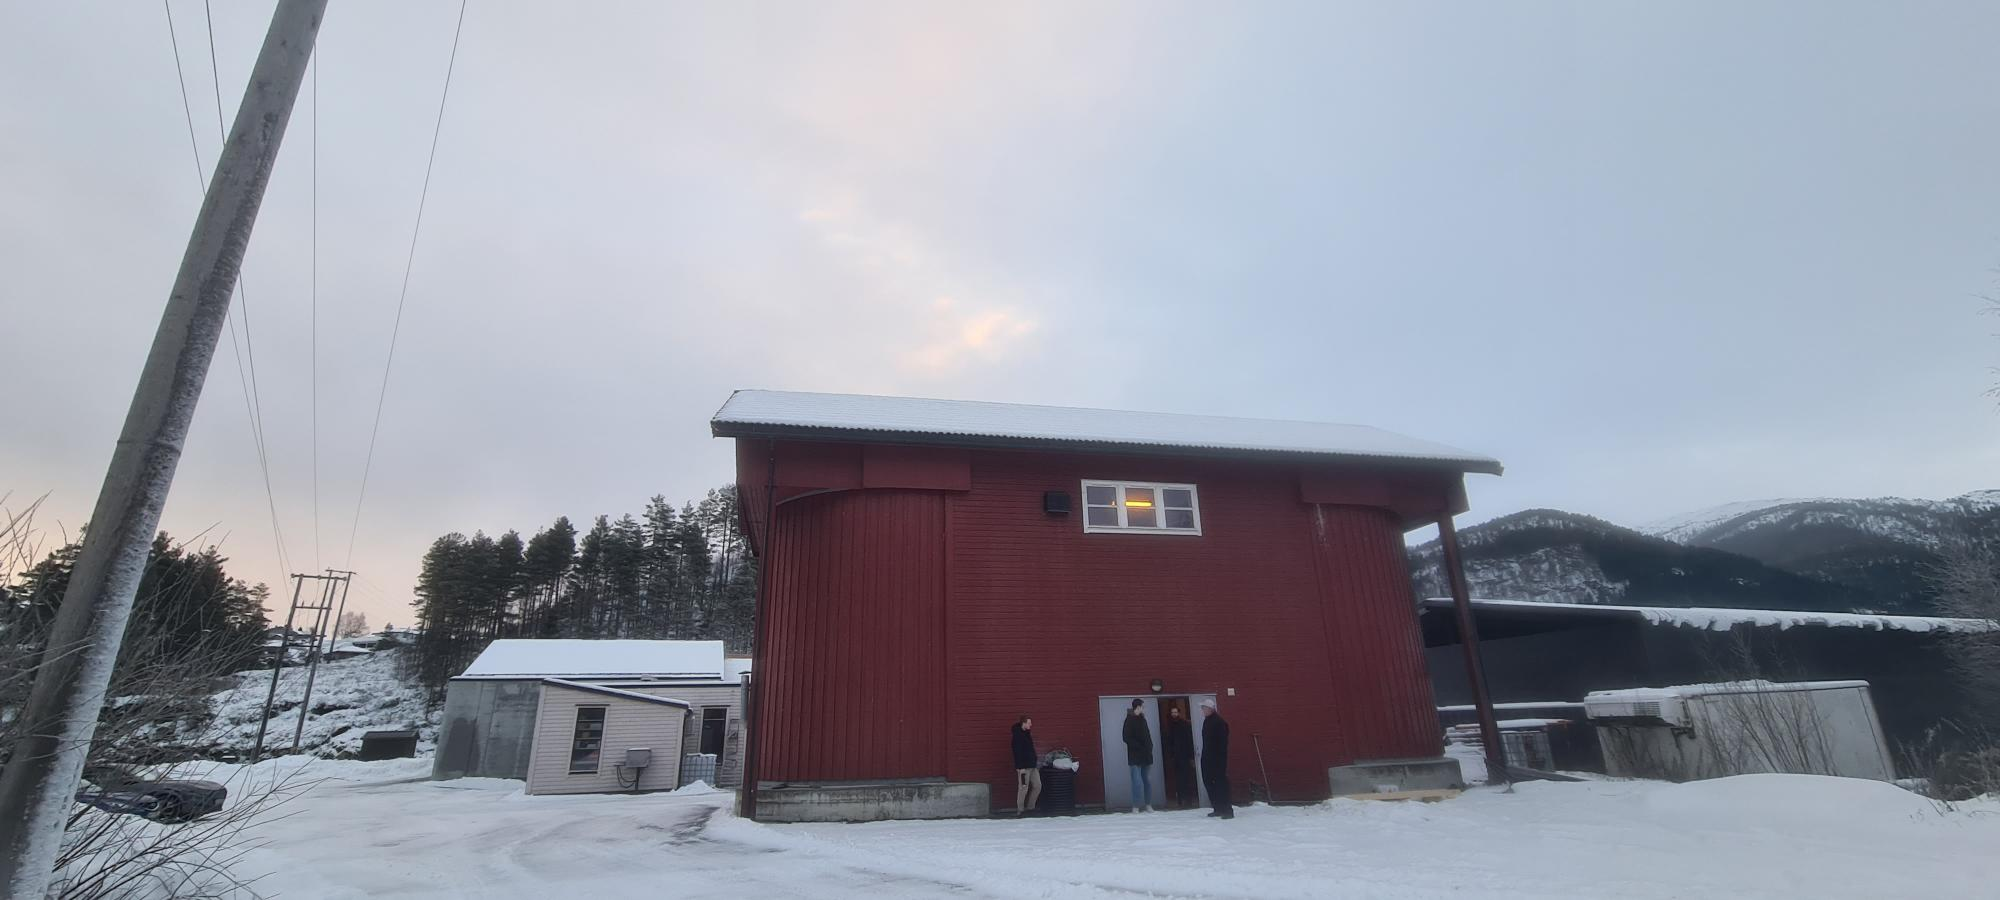
\includegraphics[width=1\textwidth]{Bilder/SandeGjennomgang.jpg}
    \caption{Bilete frå første gjennomgangen av anlegget}\label{fig:Bilete Gjennomgang}
\end{figure}

\begin{center}
    \textit{Foto: Håvar Dankel}
\end{center}

\newpage

\subsection{Anbefalingar av sensorikk}

For å betre anlegget og styresystemet ytterlegare vil det vere nyttig å få inn meir instrumentering. 
Auka sensorikk vil forbetre styresystemet ved å samle meir og nøyaktig data om tilstanden og ytelsen til systemet. 
Med meir data vil styresystemet bli meir automatisk og vil kunne tilpassast varierande forhold meir effektivt. 
Systemet vil og ha moglegheita til å oppdage avvik og agere tidlegare utan manuelle inngrep, noko som igjen aukar automasjonsevna.

Basert på vår nyerfarte kunnskap av annlegget og styresystemet presenterer vi ein
anbefaling på oppgradering av instrumentering som ville forbetre reinseanlegget. 
Sjølv om all sensorikk vil være verdifull, har vi vurdert kost-nytte og anbefaler kun sensorikk som vil gi tilstrekkeleg verdi.

\begin{itemize}
    \item \textbf{Strøymingsmålar} \newline
        Strøymingmålar i anlegget vil gi nøyaktige tall på mengder vatn som er i anlegget.
        Dette vil gi bedre kontroll på aktivering av høgbelastningsmodus og kontroll og rapportering av driftsdata.
        Fleire strøymningsmålarar er moglege men minimumsanbefaling er vatn inn og ut av anlegget.
    \item \textbf{Energimåling} \newline
        Måling av energi vil gi moglegeit å analyse energiforbruket for å redusere kostnadar og effektivisere prosessar.
        Komponentspesefikk energimåling kan også brukast til overvåking av utstyr for å oppdage slitasje og feil.
    \item \textbf{Reaktormålingar} \newline
        Oksygen, PH og temperatur er alle kritiske verdiar for å oppnå god biologisk reinsing i reaktorane. \newline
        Ved å ha kontroll på desse parameterane vil reaktoren kunne finjusterast for å effektivitere den biologiske reinseprosessen.
    \item \textbf{Tilbakemeldingar} \newline
        Anlegget har begrensa tilbakemeldingar på utstyr, spesielt ingen innan ventilstyring.
        Tilbakemelding er essensielt for prosesstyring, feiloppdagelse og sikkerheit.
        Utan tilbakemeldingar er reinseanlegget meir sårbar for feil som ikkje blir oppdaga før det er for seint 
        og slike situasjonar vil kunne resultere i nedetid, overlaup og andre utilsikta hendelser.
    \item \textbf{Forbetra nivåmåling} \newline
        Ei forbetring av dei akutelle nivåmålingane i anlegget vil gi meir nøyaktige mål på slammengde og slamnivå i reaktorane.
        Det vil då være mogleg å finne det eksakte skilljet mellom slam og reinsa vatn etter ein sedimenteringssekvens som igjen
        gir bedre oversikt over tilstanden til den biologiske reinseprosessen.
    \item \textbf{Oppløysning} \newline
        Oppløysning på analoge målingar er idag kunn 0-1000 bit på 4-20mA.(Sjå datablad appendix xXx) \newline
        Oppgradering av måleoppløysning vil gjere kvar eksisterande og nye analoge målingar
        meir nøyaktig som igjen gir moglegheit for betre styring og regulering.
\end{itemize}
\newpage

